% Four-cut summary, drawn from the logged numbers.
% The script's own summary PNG covers only the three cuts of one process,
% because cut 1 was run separately; this figure carries all four.
\begin{figure}[htbp]
\centering
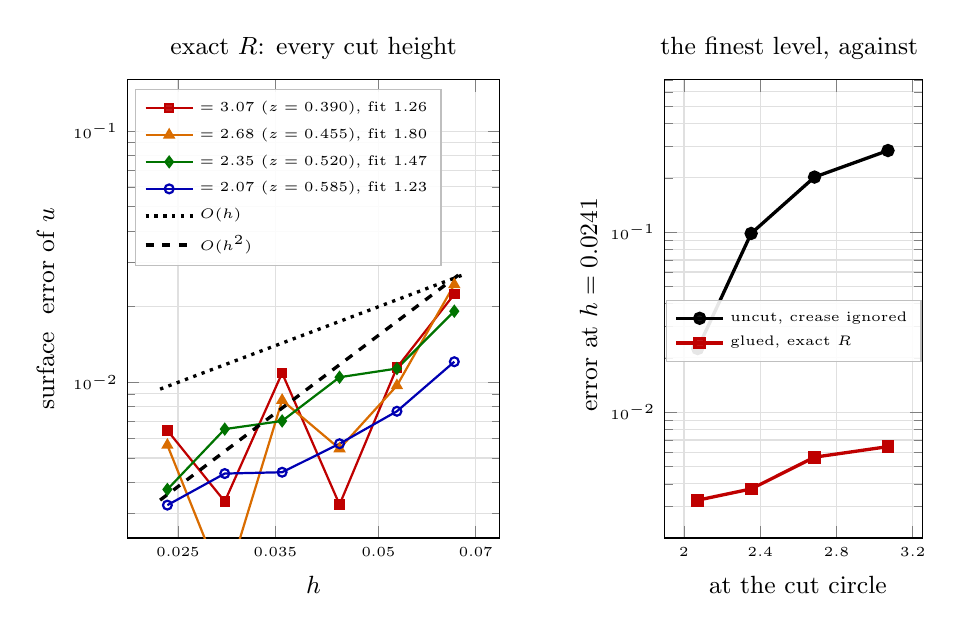
\begin{tikzpicture}

\begin{loglogaxis}[
  name=left,
  width=0.52\textwidth, height=7.4cm,
  xlabel={$h$}, ylabel={surface $\Linf$ error of $u$},
  title={\small exact $R$: every cut height},
  title style={yshift=-2pt},
  legend style={font=\tiny, at={(0.02,0.98)}, anchor=north west,
                draw=black!25, fill=white, fill opacity=0.9,
                text opacity=1, legend columns=1, row sep=0.5pt},
  legend cell align=left,
  xmin=0.021, xmax=0.076, ymin=2.4e-3, ymax=0.16,
  grid=both, grid style={black!12},
  tick label style={font=\tiny}, label style={font=\small},
  xtick={0.025,0.035,0.05,0.07},
  xticklabels={0.025,0.035,0.05,0.07},
]

\addplot[red!75!black, thick, mark=square*, mark size=1.5]
  coordinates {
    (0.065,2.244e-2) (0.053300,1.145e-2) (0.043706,3.261e-3)
    (0.035839,1.089e-2) (0.029388,3.356e-3) (0.024098,6.436e-3)};
\addlegendentry{$\dk=3.07$ ($z=0.390$), fit 1.26}

\addplot[orange!85!black, thick, mark=triangle*, mark size=1.8]
  coordinates {
    (0.065,2.451e-2) (0.053300,9.706e-3) (0.043706,5.444e-3)
    (0.035839,8.485e-3) (0.029388,1.516e-3) (0.024098,5.624e-3)};
\addlegendentry{$\dk=2.68$ ($z=0.455$), fit 1.80}

\addplot[green!45!black, thick, mark=diamond*, mark size=1.8]
  coordinates {
    (0.065,1.920e-2) (0.053300,1.135e-2) (0.043706,1.048e-2)
    (0.035839,7.020e-3) (0.029388,6.515e-3) (0.024098,3.747e-3)};
\addlegendentry{$\dk=2.35$ ($z=0.520$), fit 1.47}

\addplot[blue!70!black, thick, mark=o, mark size=1.6]
  coordinates {
    (0.065,1.208e-2) (0.053300,7.672e-3) (0.043706,5.697e-3)
    (0.035839,4.387e-3) (0.029388,4.334e-3) (0.024098,3.245e-3)};
\addlegendentry{$\dk=2.07$ ($z=0.585$), fit 1.23}

\addplot[black, dotted, very thick, domain=0.0235:0.067, samples=2]
  {2.6e-2*x/0.065};
\addlegendentry{$O(h)$}

\addplot[black, dashed, very thick, domain=0.0235:0.067, samples=2]
  {2.6e-2*(x/0.065)^2};
\addlegendentry{$O(h^2)$}

\end{loglogaxis}

\begin{semilogyaxis}[
  name=right, at={(left.east)}, anchor=west, xshift=2.1cm,
  width=0.40\textwidth, height=7.4cm,
  xlabel={$\dk$ at the cut circle},
  ylabel={$\Linf$ error at $h=0.0241$},
  ylabel style={yshift=-2pt},
  title={\small the finest level, against $\dk$},
  title style={yshift=-2pt},
  legend style={font=\tiny, at={(0.5,0.52)}, anchor=north,
                draw=black!25, fill=white, fill opacity=0.9,
                text opacity=1},
  legend cell align=left,
  xmin=1.9, xmax=3.25, ymin=2e-3, ymax=0.7,
  grid=both, grid style={black!12},
  tick label style={font=\tiny}, label style={font=\small},
  xtick={2.0,2.4,2.8,3.2},
]

\addplot[black, very thick, mark=*, mark size=1.8]
  coordinates {(2.0720,2.255e-2) (2.3525,9.824e-2)
               (2.6849,2.020e-1) (3.0703,2.836e-1)};
\addlegendentry{uncut, crease ignored}

\addplot[red!75!black, very thick, mark=square*, mark size=1.7]
  coordinates {(2.0720,3.245e-3) (2.3525,3.747e-3)
               (2.6849,5.624e-3) (3.0703,6.436e-3)};
\addlegendentry{glued, exact $R$}

\end{semilogyaxis}

\end{tikzpicture}
\caption{All four cut heights. Left: the surface $\Linf$ error of the
  glued solve with the exact rotation, against $h$. The uncut baseline is
  left out of this panel, because it is two orders of magnitude higher;
  it appears in Figure~\ref{fig:cut039} and in the right panel here. All
  four glued curves sit between the $O(h)$ and $O(h^2)$ guides, and all
  four zigzag. Right: the error at the finest level, against the
  curvature mismatch $\dk$. Both the baseline and the glued solve order
  monotonically by $\dk$, although the \emph{fitted slopes} do not ---
  see the text below.}
\label{fig:cutsummary}
\end{figure}
